\chapter{Approach}
\label{chp:Approach}
To identify the right domain size and boundary conditions, I will conduct 2D spinning circle simulations at $\Omega^{\ast} = 1, 3$ with periodic and symmetric boundary conditions. The three different domain heights that will be tested are $40D, 80D, 120D$. The main purpose of the $\Omega^{\ast}=1$ cases is to find which boundary conditions and domain size satisfy our needs, since our parameter sweep will occur at $\Omega^{\ast}=1$. We will see at what domain size are the values of drag insensitive to changes in boundary conditions and domains height. The main purpose of the $\Omega^{\ast}=3$ cases is to identify the physics, since the effects will be obvious. We will plot the surface pressure distribution of the circles to see how the pressure distribution shifts. 

To validate the Schwarz-SEM (Neknek) framework for spinning ellipses, I will run simulations in homogeneous flow. I will compare the drag and lift values to those of \cite{lu_flow_2018} and \cite{lua_rotating_2018}. To validate the framework for static circles in stratified flows I will run monodomain and Schwarz-SEM cases of static circular cylinders in a stratified cross-flow. I will compare the drag and lift coefficients. I will conduct mesh independence tests by finding an edge case and running a simulation with increased polynolial order and decreased polynomial order to see it make a difference in drag and lift. 

To find the effect of stratification and spin on flow I will run a parameter sweep of spinning and nonspinning circular cylinders and spinning ellipses of varying aspect ratios. 
\section{Governing equations {\&} problem setup}
\label{section:governing_equations_and_setup}
We want to ascertain the effect shape, spin, and stratification have on flow. We start by discussing how we account for stratification. We use the same setup used by \cite{fischer_nek5000_nodate} in the Nek5000 user guide. We relate the density $\rho$ at a given height $\mathbf{x}$ to the constant background density $\rho_0$, $\rho = \rho_0 + \rho ' (\mathbf{x},t)$. The term $\rho'$ is the perturbation density, which we will assume to have a linear profile. This means the overall density $\rho$ has a linear profile. To account for the buoyancy forces from stratification, we utilize the Boussinesq approximation. The Boussinesq approximation is where effects of density stratification are only applied to the forcing term, or terms multiplied by gravity forces in this case, in the governing equations. The Boussinesq approximation also assumes $\rho_0 \gg \rho '$.
We apply the Boussinesq approximation to the nondimensional Incompressible Navier-Stokes Equations (INSE) shown in Equations \ref{eq:INSE} and \ref{eq:cont}:

\begin{equation}
    \label{eq:INSE}
    \frac{\partial\mathbf{u}}{\partial t}+\mathbf{u}\cdot\nabla\mathbf{u}=-\nabla p+\frac{1}{\Rey}\nabla^2\mathbf{u}-\frac{1}{{Fr}^2} (\rho^\prime\ -\ y )\hat{y}
\end{equation}

\begin{equation}
    \label{eq:cont}
    \nabla \cdot \textbf{u} = 0
\end{equation}
We also solve the transport equation in \ref{eq:density transport}, which is the material derivative of the perturbation density set equal to a diffusion operator.  
\begin{equation}
    \label{eq:density transport}
    \frac{\partial\rho '}{\partial t}+\mathbf{u}\cdot\nabla\rho'=\frac{1}{\Pran \Rey}\nabla^2\rho '
\end{equation}
The three nondimensional numbers that appear in the equations above are defined as such:
\begin{equation}
    \Rey = \rho_0 \frac{U D}{\mu}, \Pran = \rho_0 \frac{\kappa}{\mu}, Fr^{-2}=\frac{gD^2}{\rho_0 U^2}|\rho^{\prime}_{y,0}|
\end{equation}
where $\rho^{\prime}_{y,0}$ is the density gradient, which in this case is constant. The term $U$ is the velocity scale, $D$ is the length scale, which will be discussed more later. Dynamic viscosity, also known as momentum diffusivity, is represented by $\mu$, and $\kappa$ is the diffusivity of the property that is causing the stratification, which in this case is thermal diffusivity. Because the densimetric Froude term $Fr^{-2}$ is slightly clunky, often it is substituted with the Richardson number $Ri \coloneqq Fr^{-2}$. We are able to extract the physical quantity called the Brunt–Väisälä frequency defined as
\begin{equation}
    \label{eq:NBV}
    N_{BV} \coloneqq \bigg( \frac{g}{\rho_0} \rho^{\prime}_{y,0} \bigg)^{1/2}    
\end{equation}
With nondimensionality and setting $U = 1$ and $D = 1$, the Brunt–Väisälä frequency can be redefined in terms of nondimensional parameters to yield
\begin{equation}
    \label{eq:nondim NBV}
    N_{BV} = Ri^{1/2} = Fr^{-1}
\end{equation}
We observe that with higher stratification, we get higher frequencies of oscillation. 
To understand the effect of shape, we look at three different aspect ratios. A circle is included to allow for benchmarking purposes with literature since a sufficient number of studies have looked at spinning circles. It is shown that the horizontal dimension, $a_x$ of the body is held constant, and this dimension is what is used for the length scale used in the Reynolds number $\Rey = \rho_0 \frac{U D}{\mu}$ , where $D = 2a_x$. The other dimension $a_y$ is varied to achieve the different aspect ratios. The aspect ratio is defined as $AR = a_y/a_x$. Figure \ref{fig:flow setup} show the aspect ratios of interest for this study. 
Now we introduce spin into our setup. We follow the conventions of \cite{mittal_direct_2020} and define our nondimensional rotational velocity as $\Omega^{\ast} = \tilde{\Omega}D/2 U_{\infty}$, where $\tilde{\Omega}$ is the rotational velocity in radians per unit time. Figure \ref{fig:flow setup} shows how the ambient flow, rotation, and axes are related. The axis of rotation, which in this case is the out-of-plane z-axis, is normal to the flow. The flow occurs in the x-direction. 
\begin{figure}
    \centerline{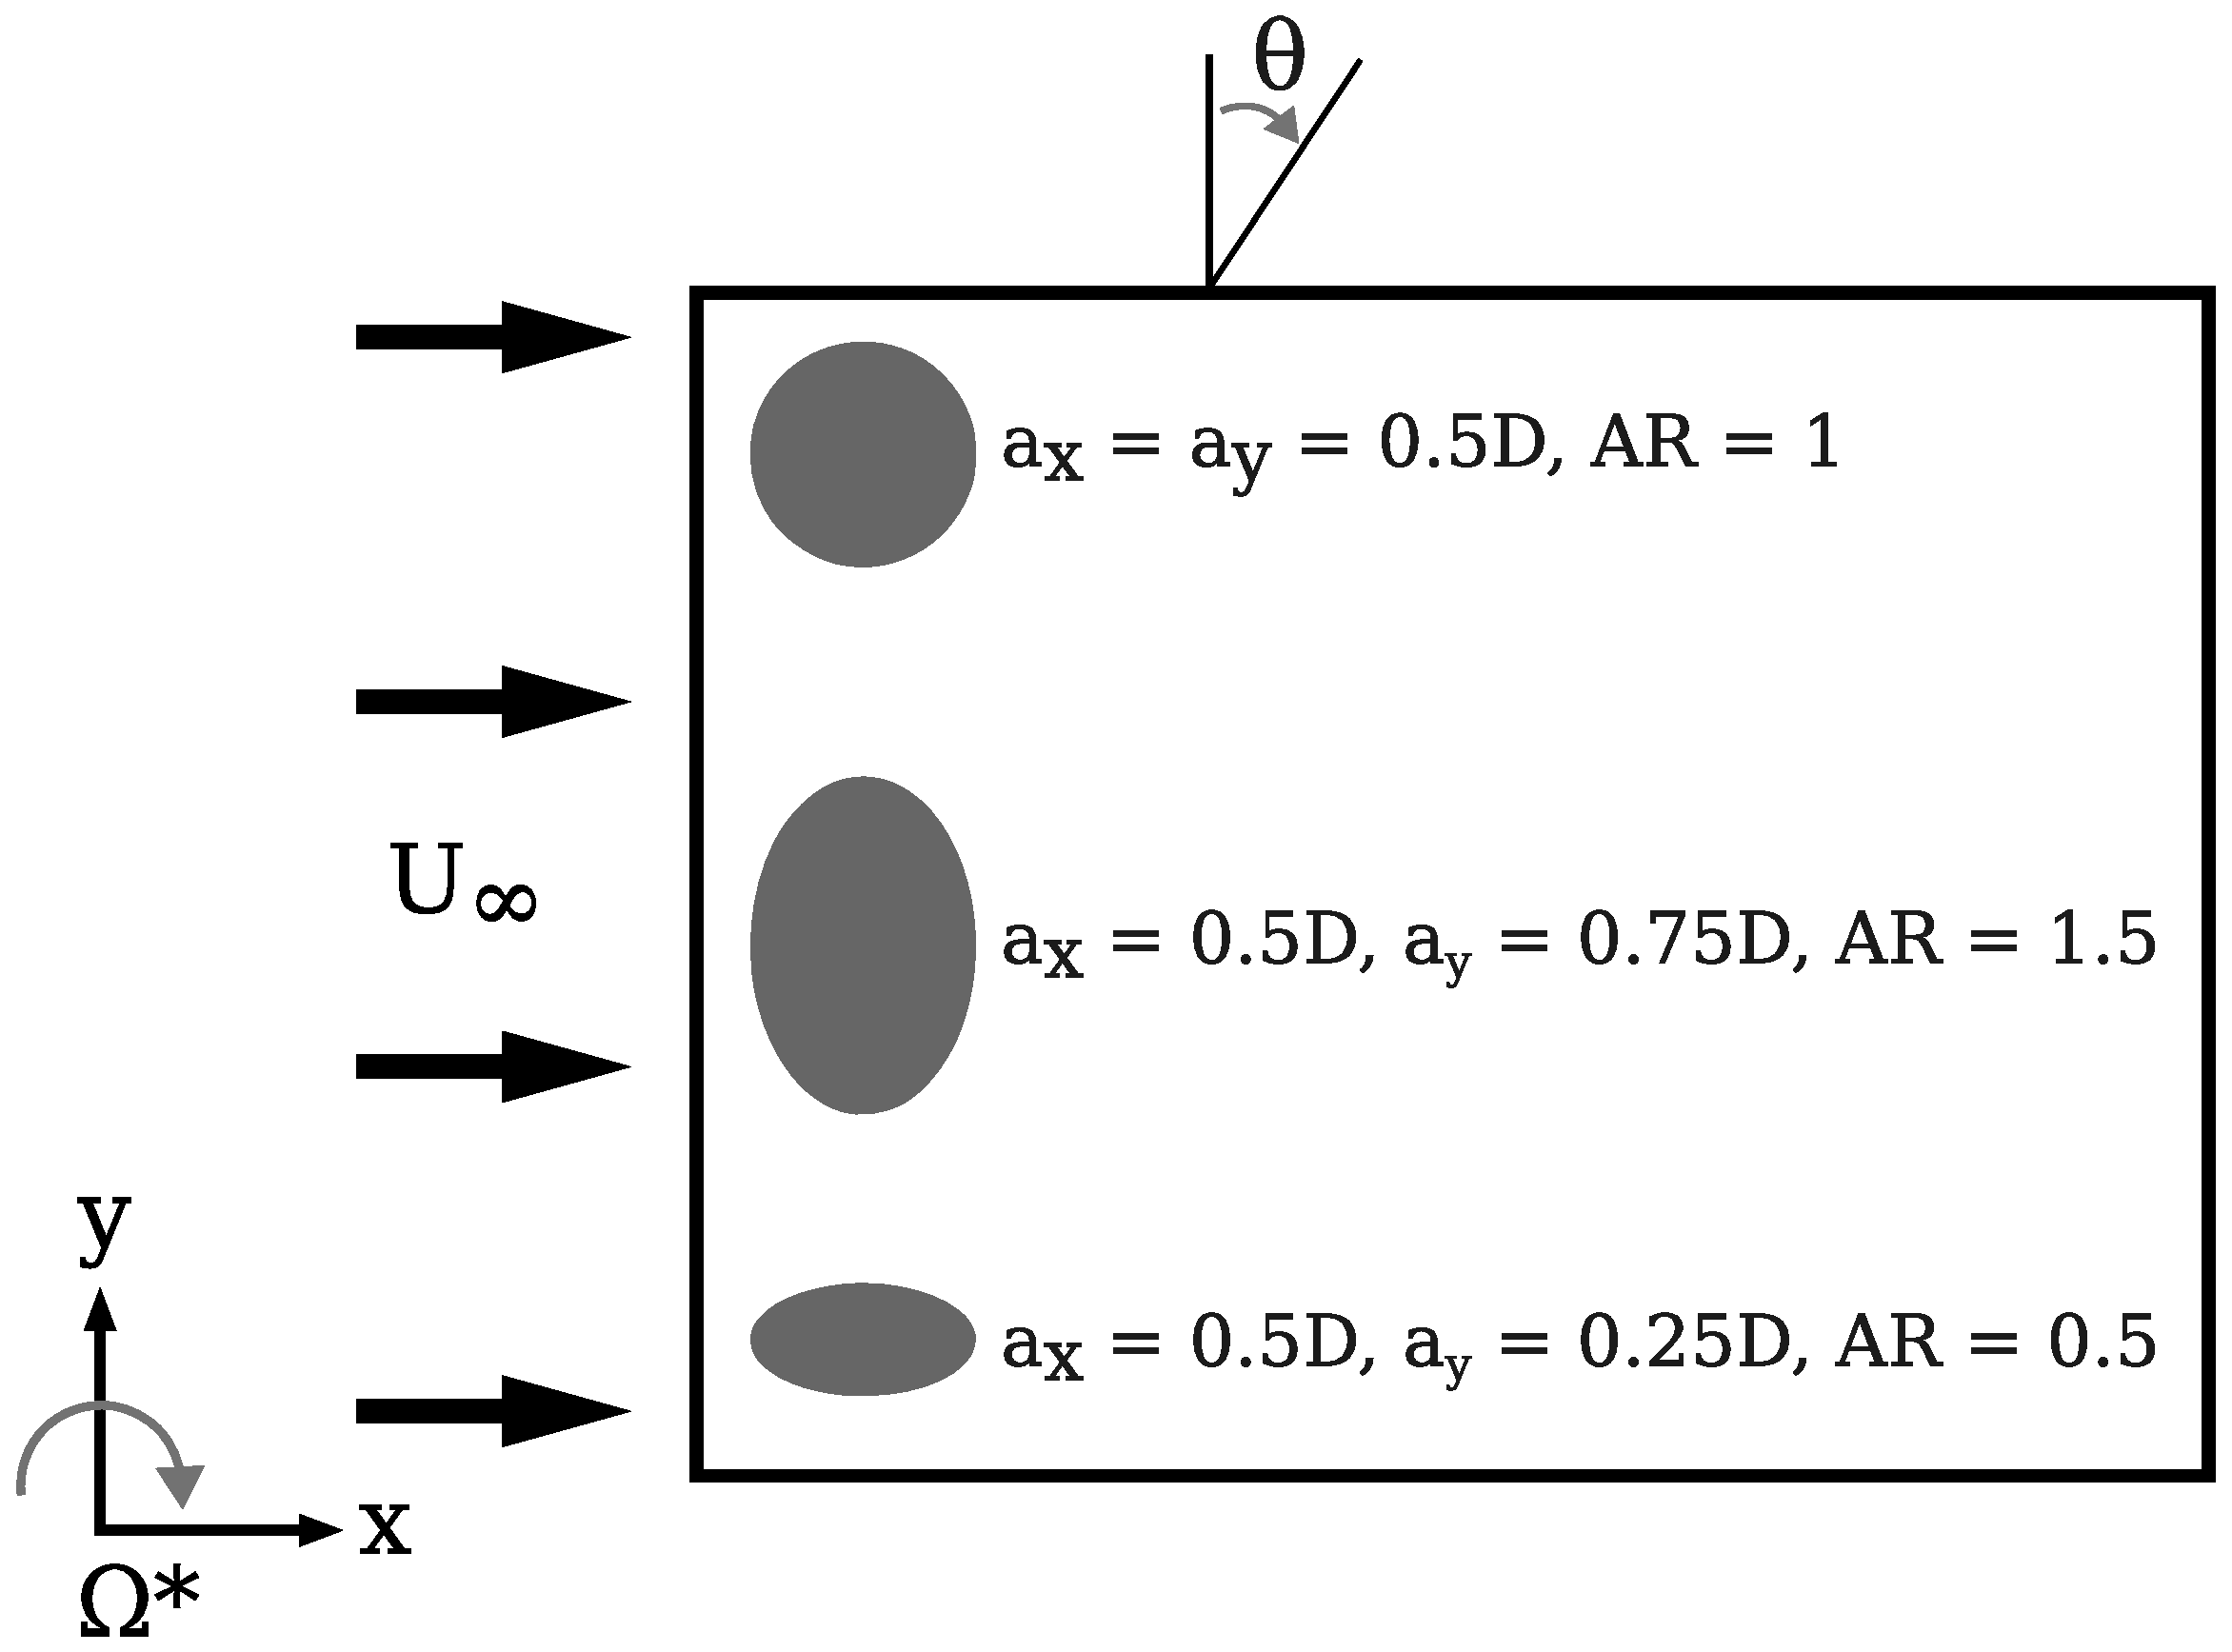
\includegraphics[width=.6\textwidth]{flow_setup.eps}}
    \caption{Schematic showing aspect ratios of interest}
    \label{fig:flow setup}
\end{figure}

This study utilizes Spectral Element Methods to perform DNS. These methods allow for higher-order accuracy than methods used in past studies. Lagrange interpolants with Gauss-Lobatto-Legendre (GLL) quadrature are utilized. 
We consider cases at $\Rey = 120$. We do not go much higher than $\Rey = 120$ because at $\Rey >190$ flow regimes, 2D simulations do not sufficiently capture the flow features observed in 3D simulations as stated by \cite{deng_drag_2022}. We do not want to go to smaller $\Rey$ because the flows of interest occur at $\Rey > 100$. We run simulations where the stratification is a result of a linear temperature distribution, and we run simulations at a constant $\Pran = 1$. The rates of rotation of interest we will consider are $\Omega^{\ast} = 0, 1$. We compare cases with spin and no spin to observe what effect introduction of spin has on the flow. Table \ref{table:parameter_space} give the values of our parameter sweep. A few simulations will be run outside this parameter space to explore transitional flow regimes. 
\begin{table}
  \centering
  \begin{tabular}{cc}
    Parameters      & Values   \\ \hline
    $AR$   & $0.5, 1.0, 1.5$ \\
    $Fr^2$ & $0.01, 0.1, 1.0, 10.0, 100.0, \infty$     \\
    $\Rey$ & $120$  \\
    $\Omega^{\ast}$ & $0.0$ (AR = 1 \text{only}), $1.0$  \\
  \end{tabular}
  \caption{The values of interest for our parameter sweep}
  \label{table:parameter_space}
\end{table}
 \clearpage

\section{Schwarz-SEM framework}
\label{section:schwarz-SEM_framework}
Because we intend to simulate nonspherical spinning bodies, it becomes necessary to create two different meshes. We create one circular mesh which conforms to the shape of the body and rotates with the body. We utilize another static, background mesh with a circular cavity where the circular mesh is placed. There is an overlap between the two meshes to allow for data exchange. We utilize the Schwarz-SEM framework, which allows us to run simulations with multiple meshes. The Schwarz-SEM framework has its roots in the Overlapping-Schwarz (OS) methods developed by Schwarz in 1870 \cite{mittal_nonconforming_2019}. Laplace's equation was solved on two overlapping domains by interpolating interdomain boundary conditions.  

\begin{figure}\centerline{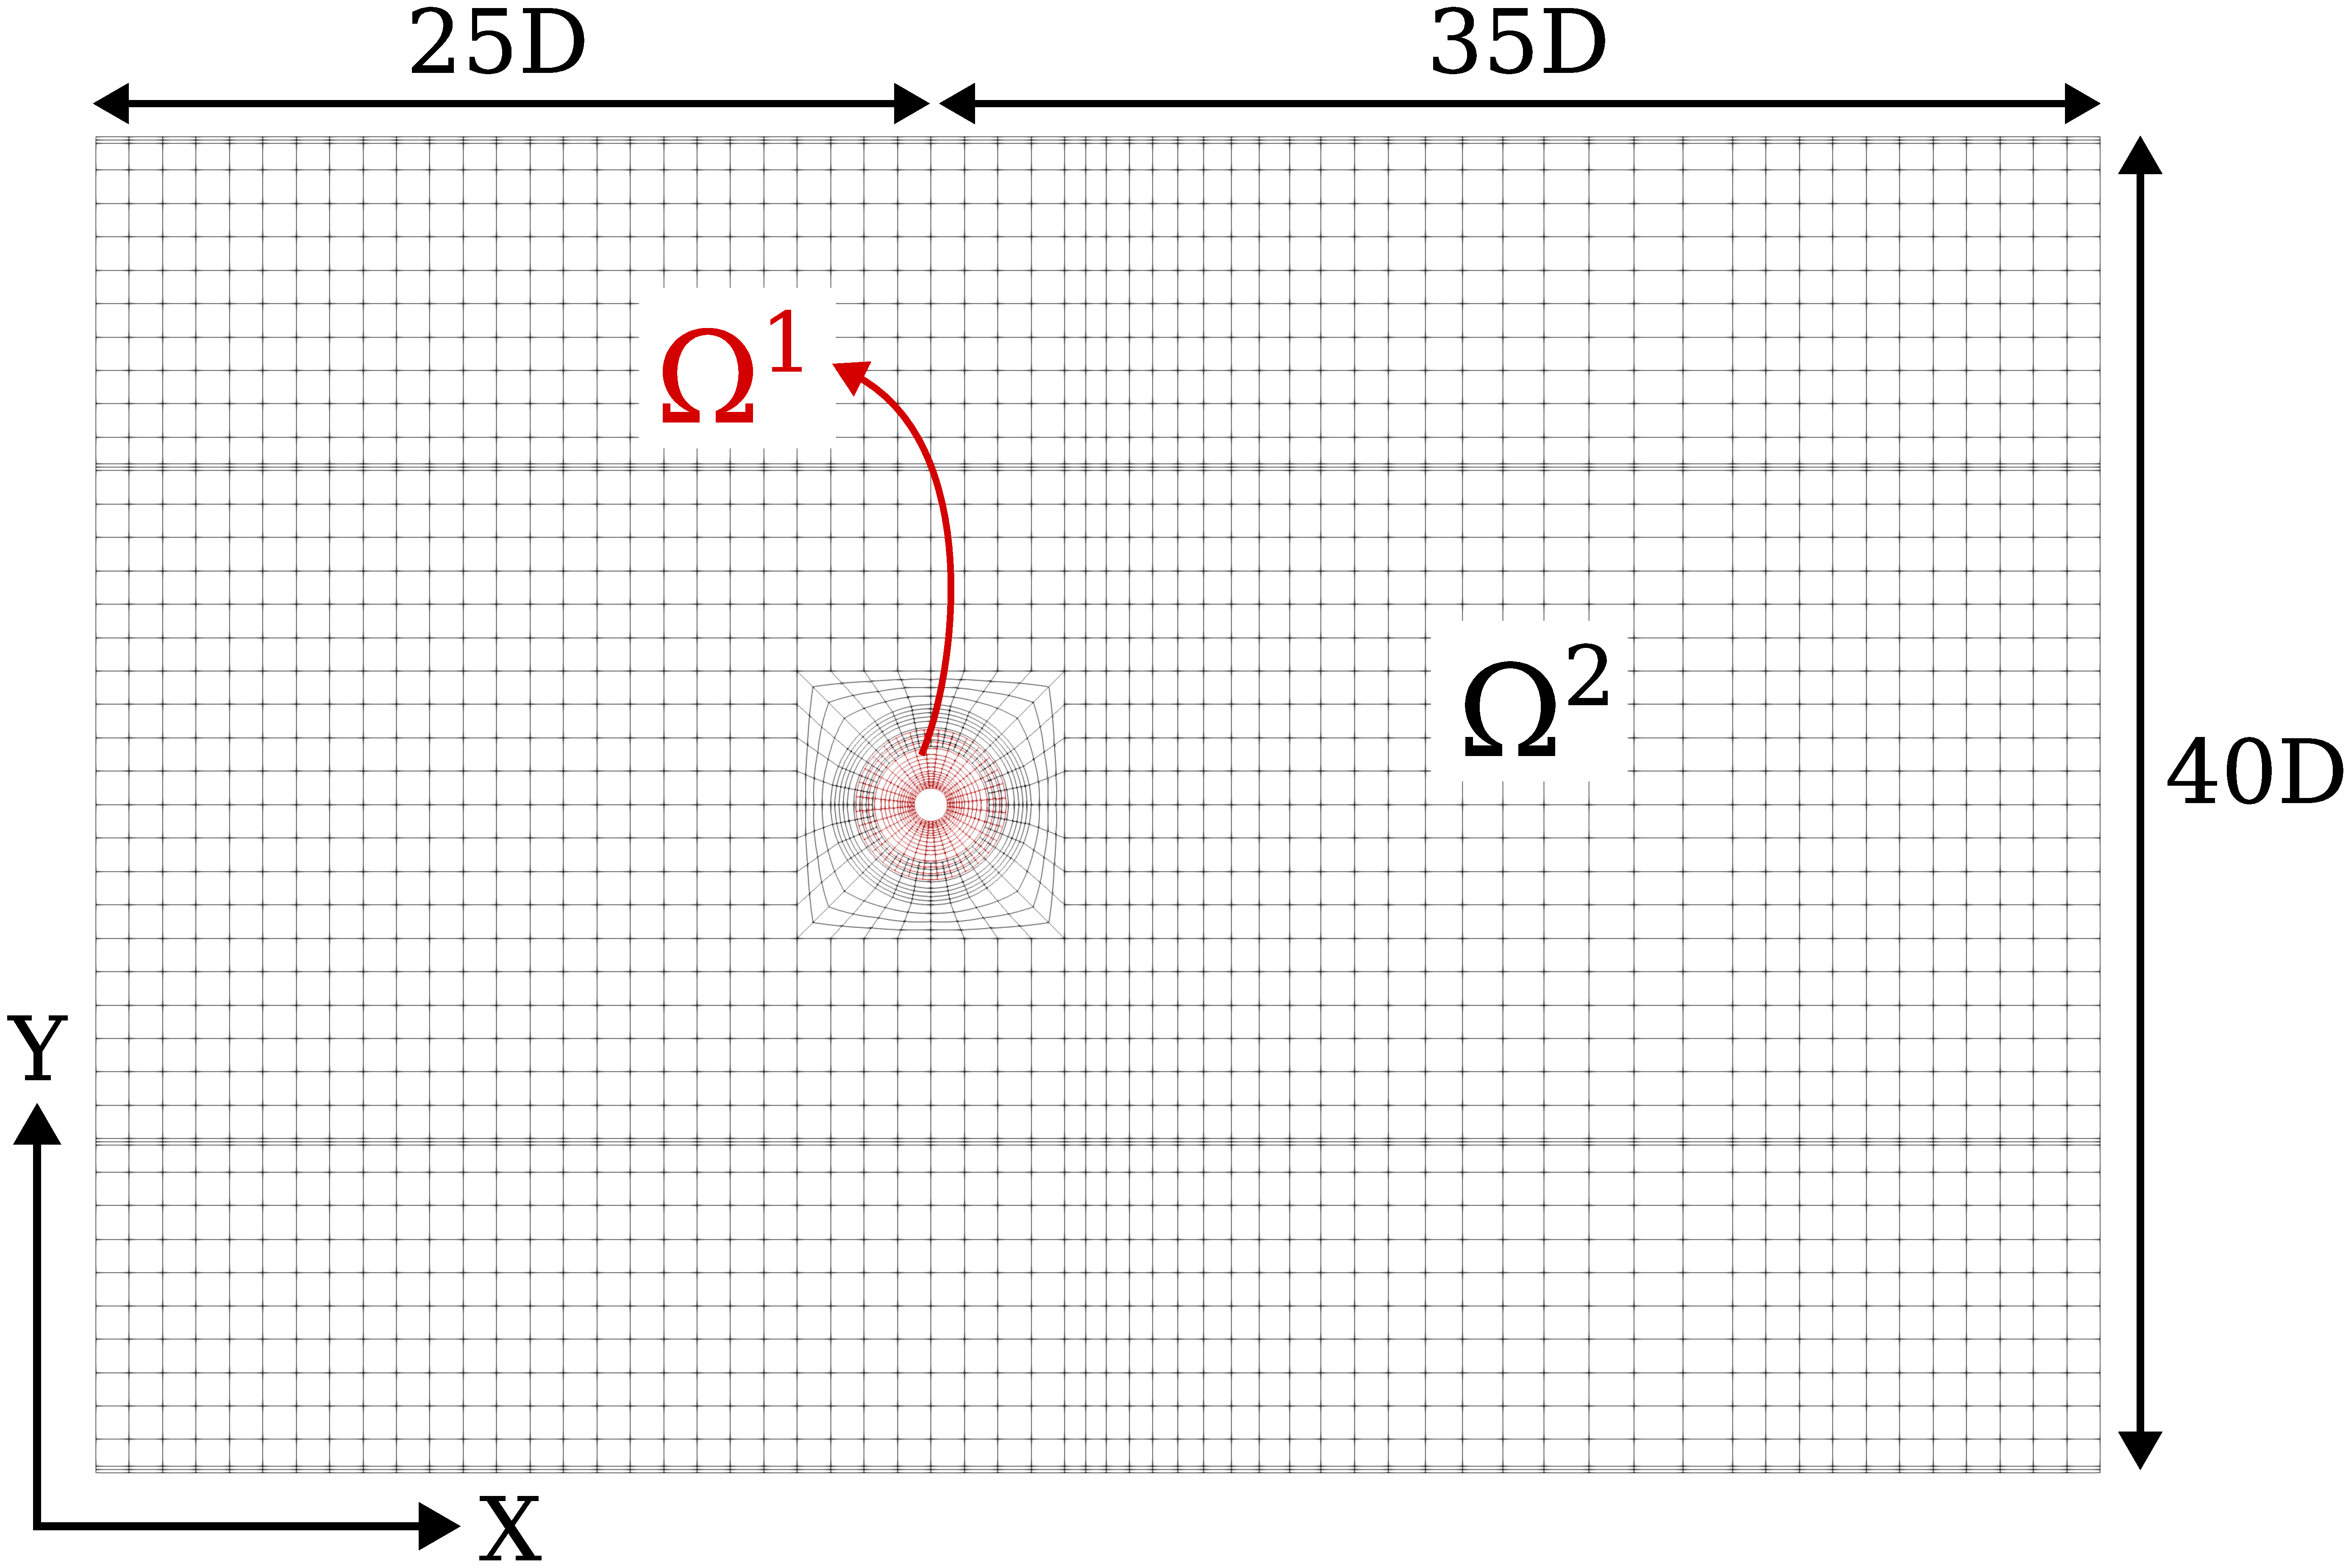
\includegraphics[width=.8\textwidth]{mesh.eps}}
    \caption{A figure showing the two meshes $\Omega^1$ and $\Omega^2$ in the Schwarz-SEM framework}
    \label{fig:mesh}
\end{figure}

In spite of the fact that the Schwarz-SEM framework was developed with the intention for use in static domains, an Arbitrary Lagrangian-Eulerian (ALE) formulation has been developed to allow for moving bodies. The implementation of the ALE formulation occurs with a modification of the convective term in Equations \ref{eq:INSE} and \ref{eq:density transport} as \cite{merrill_moving_2019} show. The advantage of using an overlapping mesh rather than a sliding mesh is we are able to retain spectral accuracy. Sliding mesh methods are limited to second-order accuracy.
For advancing in time, a semi-implicit scheme is implemented, rather than a fully implicit scheme. The reason for choosing a semi-implicit scheme is the cost of a fully implicit scheme as discussed by \cite{tomboulides_numerical_1997}. In the semi-implicit scheme, the nonlinear terms and Boussinesq forcing term are treated explicitly with \textit{k}th-order extrapolation since they would increase the cost substantially if treated implicitly. The time derivative is implicitly treated with a \textit{k}th-order backward difference formula (BDF\textit{k}) because we want to retain high-order temporal accuracy. The viscous and pressure terms are decoupled and treated implicitly through Poisson updates.\\\\
Every timestep, the boundary conditions at the interdomain boundaries are interpolated from the adjacent mesh. This occurs every timestep because the locations of the inner mesh GLL nodes change every timestep. \cite{mittal_nonconforming_2019} implemented a routine called \textit{findpts\_eval} from the library \textit{gslib} that carries out the boundary condition interpolation. Using the \textit{findpts} routine, the routine \textit{findpts\_eval} finds the corresponding element and element coordinates from the adjacent mesh.\\\\
At the interdomain boundaries, the solutions are advanced in time every timestep with EXT\textit{m} using $m$ number of preceding steps in time to increase the temporal accuracy. Higher order $m$ leads to instability, so $q$ corrector iterations are implemented every timestep, and the data is interpolated from the adjacent domain before every corrector iteration. In the case of our parameter sweep, we set $m=3$ and $q=5$ to achieve sufficient data exchange. \\\\  
The top and bottom boundaries have Neumann symmetric boundary conditions. The left boundary has a Dirichlet constant velocity inflow boundary condition, while the right boundary has a Neumann zero-pressure outflow boundary condition. Meanwhile, the surface of the cylinder has a Dirichlet no-slip wall boundary condition. The size of the domain is $60D \times 40D$, where $D$ is the length of the non-varying axis of the ellipse; the radius of the inner mesh is $2.25D$. The inner mesh consists of 512 elements, while the outer mesh consists of 3200 elements. There is an overlap of $0.5D$ between the meshes. 

\clearpage

\section{Validation}
\label{section:validation}
We start by validating our Schwarz-SEM framework against a commonly-used nonspinning circle monodomain SEM case. We ran monodomain and Schwarz-SEM simulations in domains of size 43x24. In these validation cases, our parameter space is $\{\Rey, \Pran, AR, \Omega^{\ast}\} = \{120, 1, 1, 0\}$. Figure \ref{fig:nn val} compares the drag coefficient, which is calculated as $C_D = 2F_D$. We only see a slight disagreement at $Fr^2 = 0.01$, which comes out to an error of less than $3.1\%$.  

\begin{figure}
    \centerline{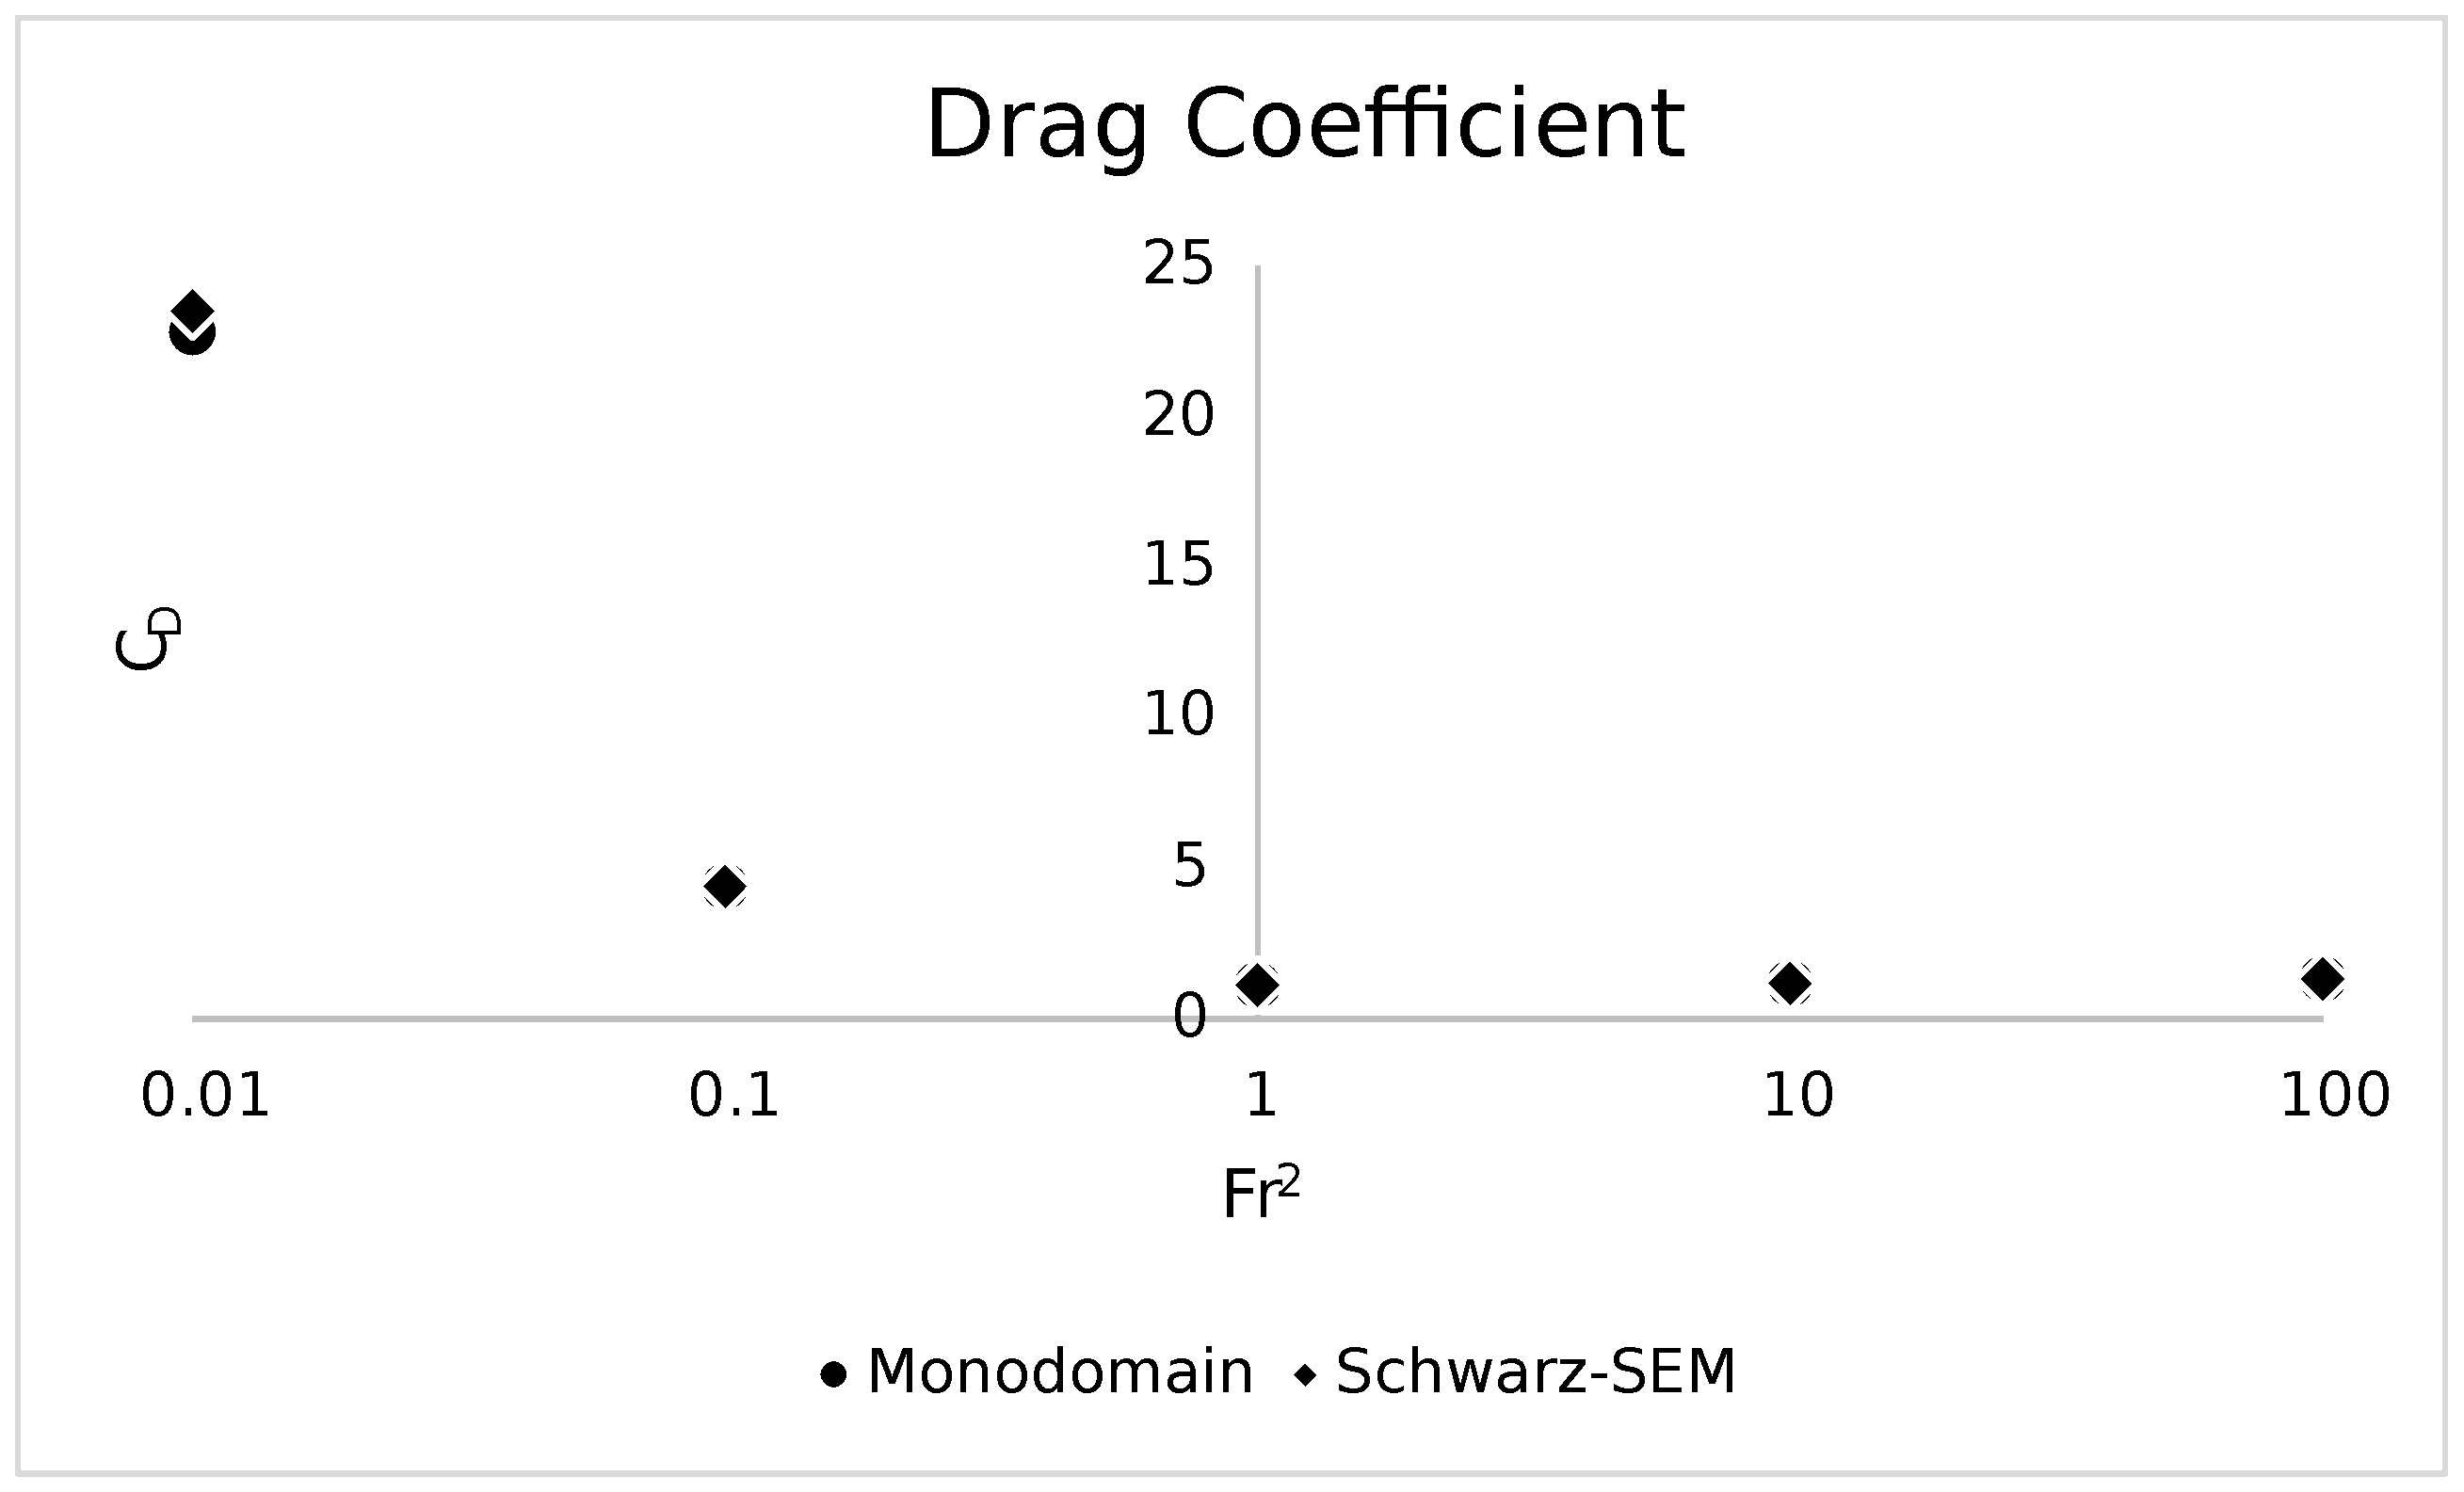
\includegraphics[width=.8\textwidth]{images/dragvalnn.eps}}
    \caption{Validation of the Schwarz-SEM framework at $\Omega^{\ast}$ for stratified flow}
    \label{fig:nn val}
\end{figure}

Now that the nonspinning stratified Schwarz-SEM for circular shapes has been validated, we move to validating the nonstratified, elliptical Schwarz-SEM framework. We compare our drag and lift results with those of two papers, Lu et al. \cite{lu_flow_2018} and Lua et al. \cite{lua_rotating_2018}. Our domain dimensions and boundary conditions matched. Figure \ref{fig:lua drag} shows the drag results between us and the two papers. Interestingly, the net thrust observed by the two papers is also observed in our results.
\begin{figure}
    \centering
    \begin{subfigure}{0.49\textwidth}
    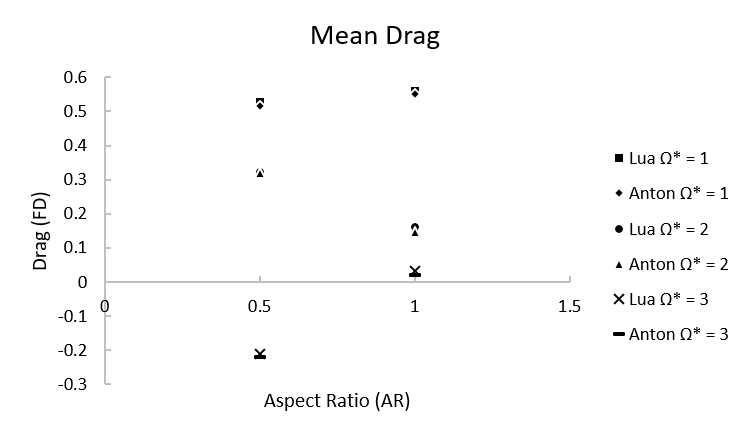
\includegraphics[width=\textwidth]{draglua.png}
    \caption{Comparison of drag results with Lua et al.}
    \label{fig:lua drag}
    \end{subfigure}
    \begin{subfigure}{0.49\textwidth}
    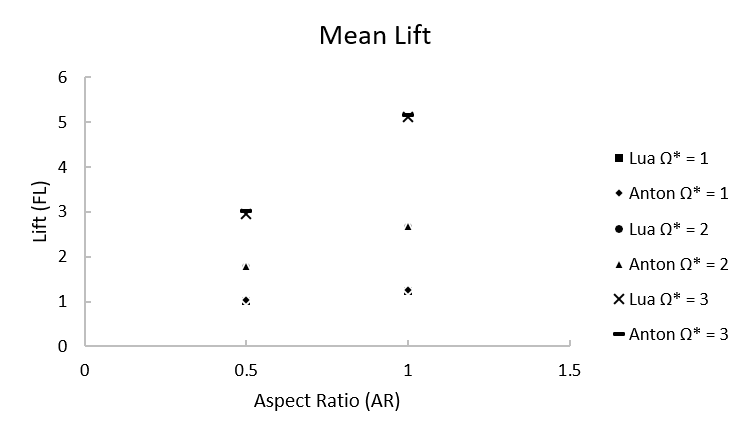
\includegraphics[width=\textwidth]{liftlua.png}
    \caption{Comparison of lift results with Lua et al.}
    \label{fig:lua lift}
    \end{subfigure}
    \caption{Comparison against Lua et al.}
    \label{fig:lua_com}
\end{figure}
While conducting these validation tests, it was found that at higher rotation rates, the drag values are more sensitive to domain size and lateral boundary conditions. This is a topic that is not discussed much in the literature; domain size and lateral boundary conditions are not given much consideration. 

Figure \ref{fig:domain_conv} shows that in the case of $\Omega^{\ast} = 3$, there is a large discrepancy in drag at height $H = 40D$ between the two boundary condition types. We also see that as we change the domain size, regardless of boundary condition, the drag also changes.  However, there is a vertical length of convergence for domain size. For the case of $\Omega^{\ast} = 3$, we observe a convergence towards a value of about $120D$. Interestingly, the variance is higher in the case of the periodic boundary conditions than the symmetric boundary conditions. The figure also shows that there is also a vertical length of convergence where the drag for the periodic and symmetric boundary condition cases converge. The required height increases with rotational velocity, as expected. 
\begin{figure}
    \centerline{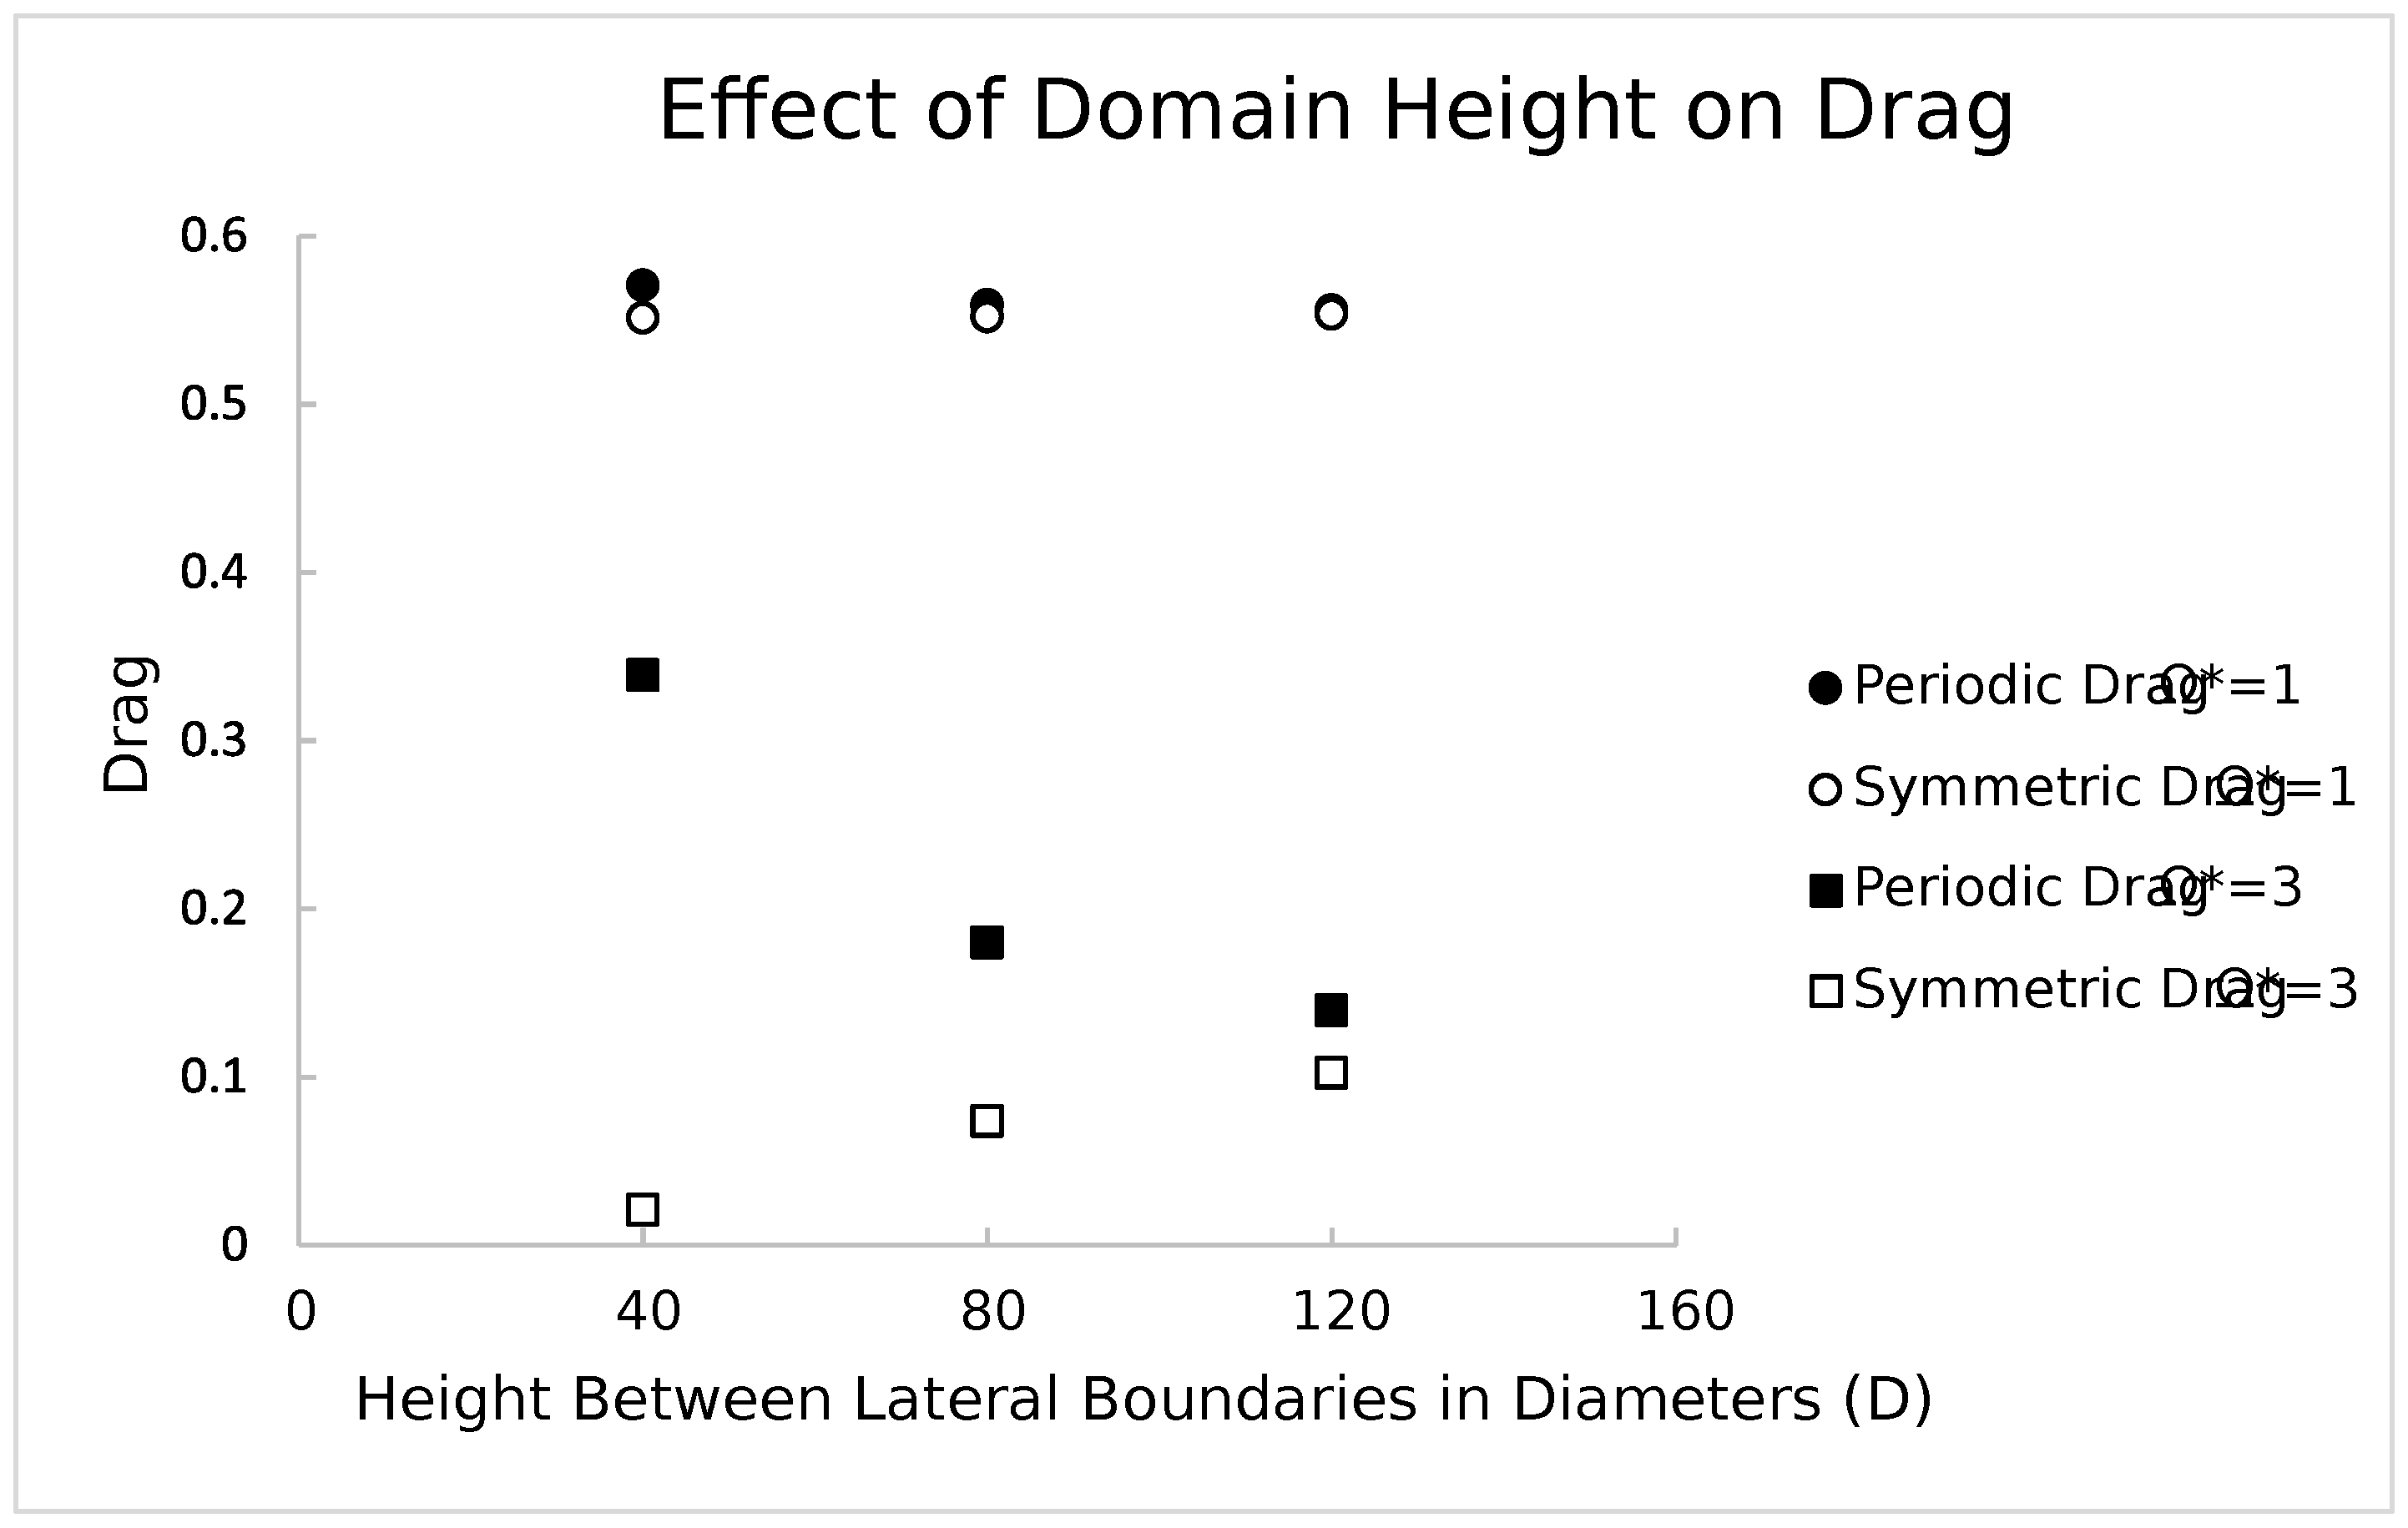
\includegraphics[width=.9\textwidth]{domain.eps}}
    \caption{At higher rotation speeds, larger domain sizes are required}
    \label{fig:domain_conv}
\end{figure}
In figure \ref{fig:per}, we see how in the case of the periodic boundary conditions, the rotation of the cylinder is able to redirect the flow down since the periodic boundary conditions allow for flow normal to the boundaries; the flow comes done from the top, further redirecting the flow. This does not happen in the case of the symmetric boundary conditions, as figure \ref{fig:sym} shows. Because there is no flow normal to the boundaries at the boundaries, there is no flow rotation like there is in the case of the periodic boundary conditions. 
\begin{figure}
    \centering
    \begin{subfigure}{0.49\textwidth}
    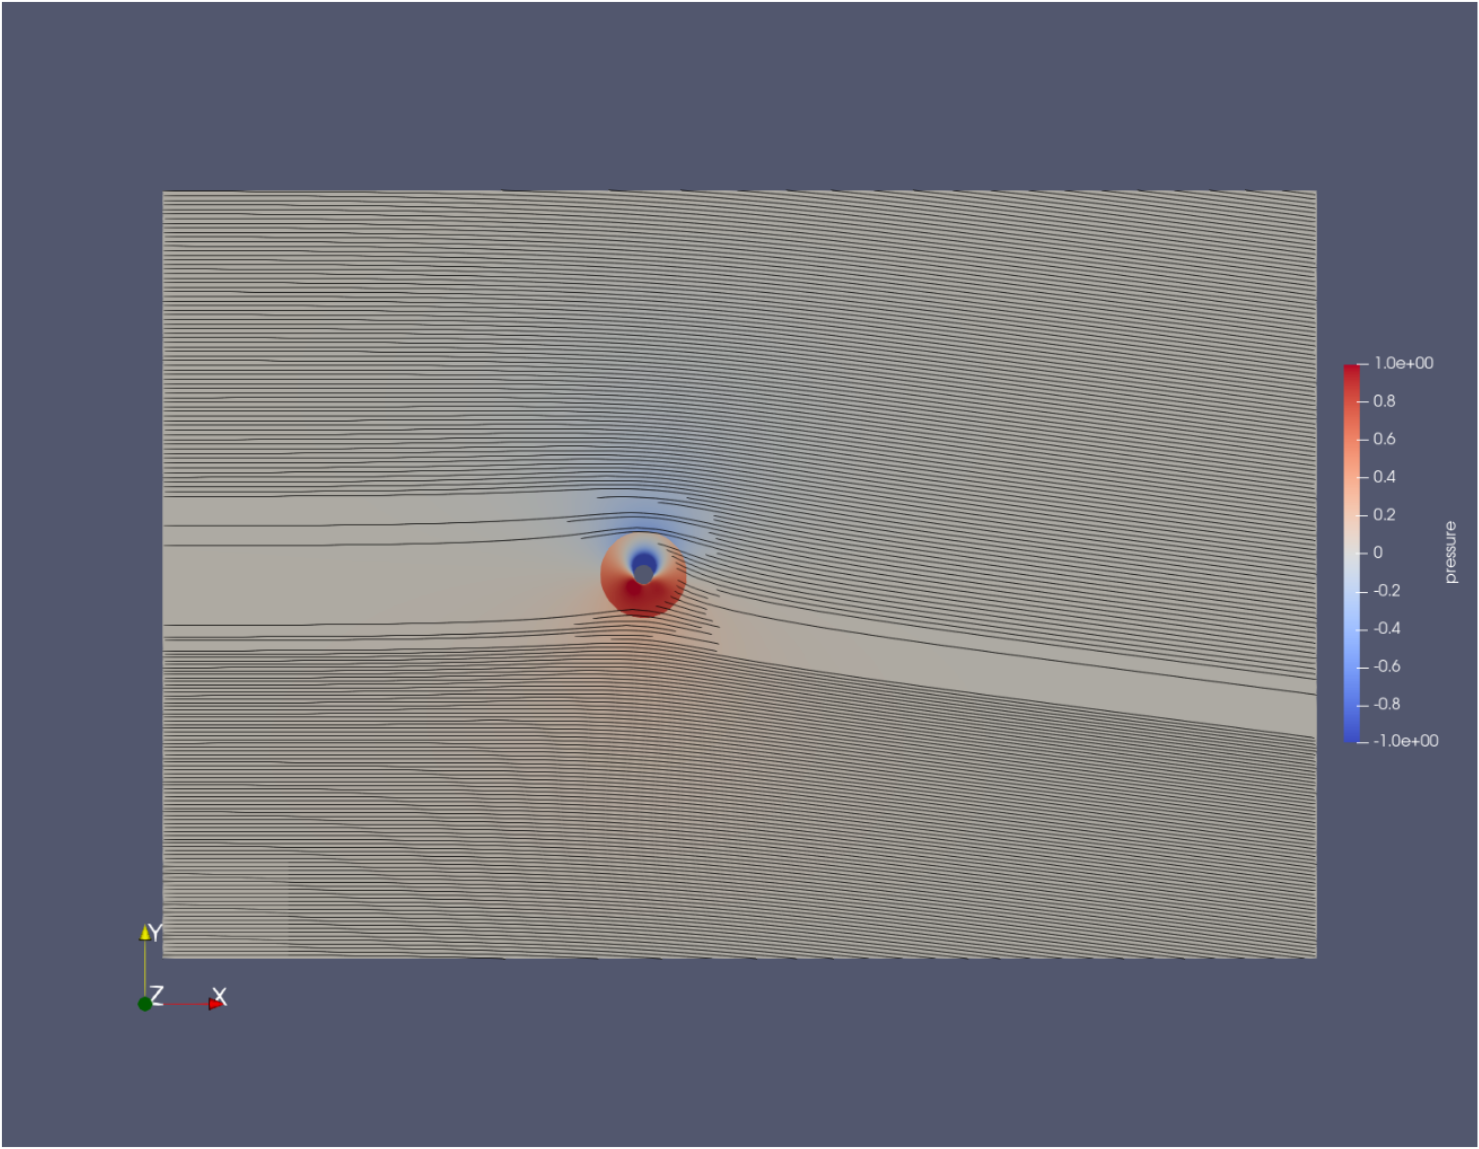
\includegraphics[width=\textwidth]{per.png}
    \caption{Periodic boundary conditions}
    \label{fig:per}
    \end{subfigure}
    \begin{subfigure}{0.49\textwidth}
    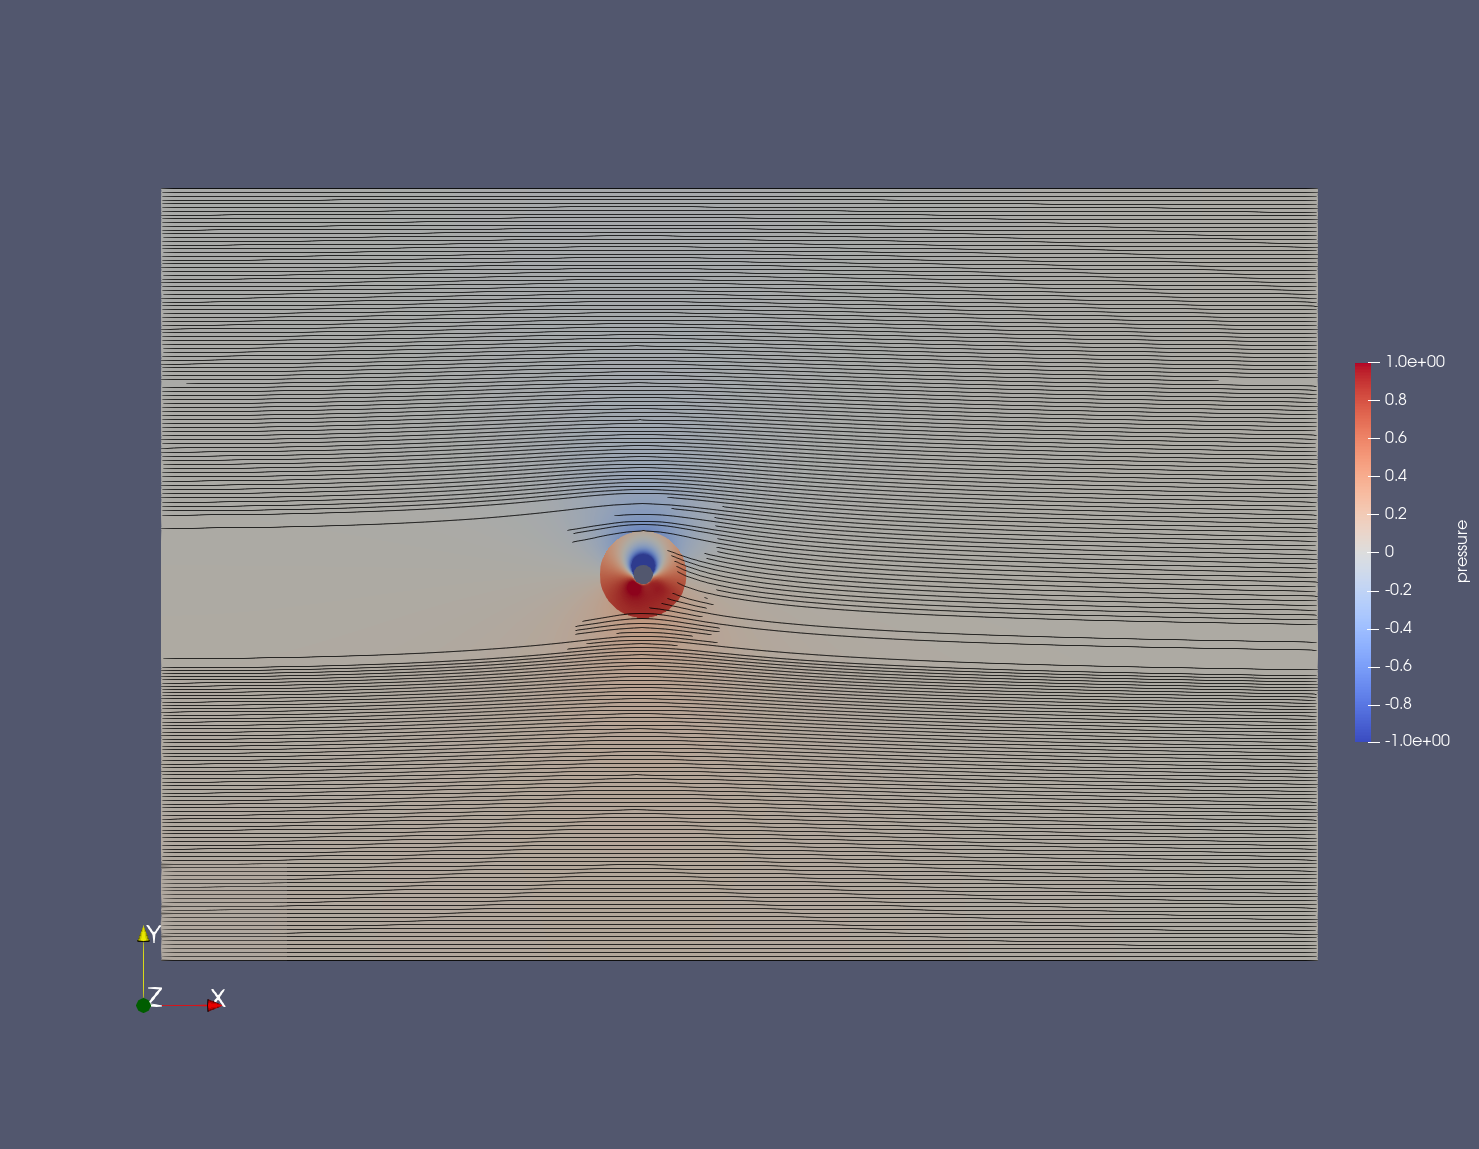
\includegraphics[width=\textwidth]{sym.png}
    \caption{Symmetric boundary conditions}
    \label{fig:sym}
    \end{subfigure}
    \caption{Pressure and streamline plots at $H = 40D$, $\Omega^{\ast} = 3$, $\Rey = 200$, aspect ratio = 1}
    \label{fig:per sym}
\end{figure}
The flow rotation in the case of the periodic boundary conditions also rotates the pressure distribution, as figure \ref{fig:polar pres} shows. The clockwise rotation of the negative pressure zone at the top creates a net increase in drag.
\begin{figure}
    \centerline{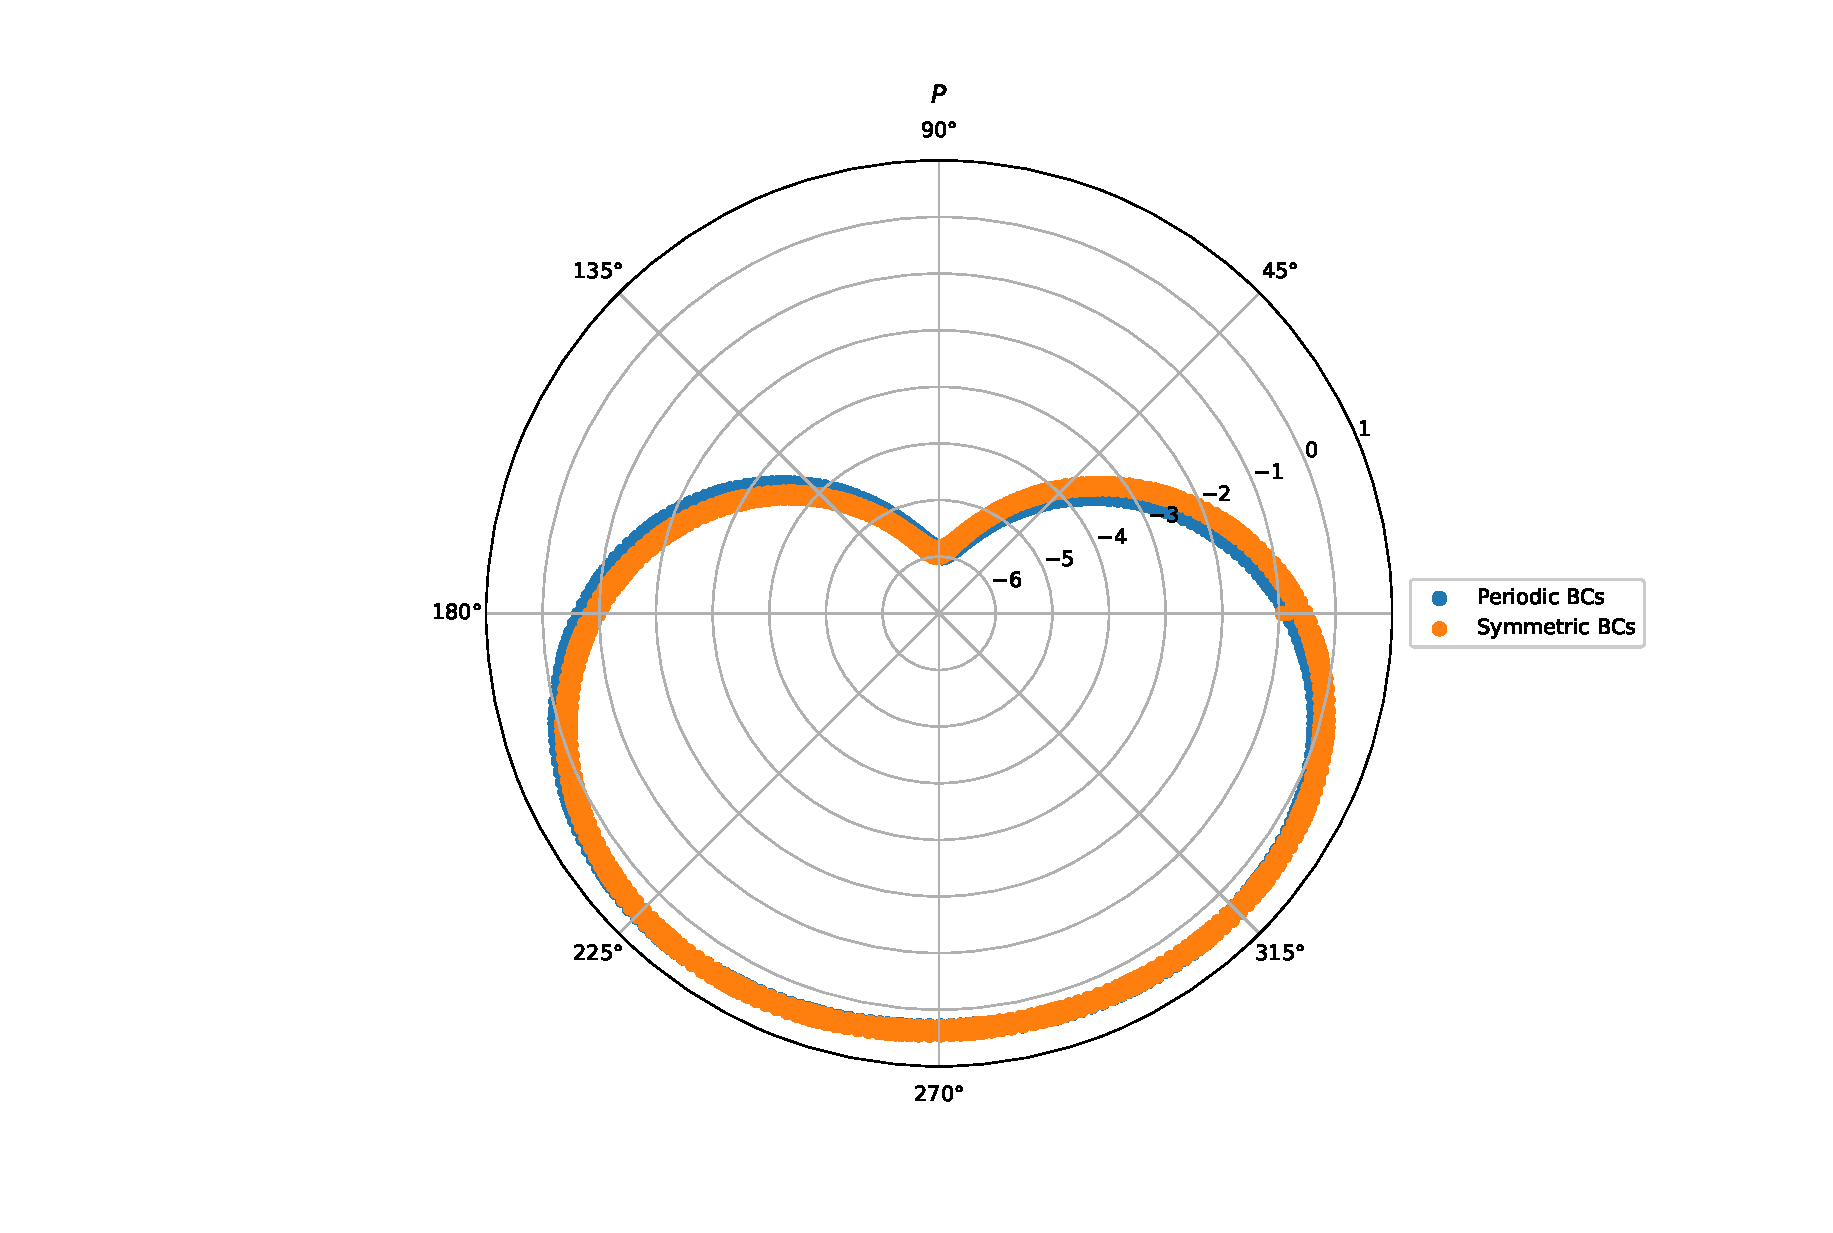
\includegraphics[width=0.9\textwidth]{polar.eps}}
    \caption{Polar plot of pressure on each surface}
    \label{fig:polar pres}
\end{figure}
The fact that the discrepancy in drag arises from the rotation of the low-pressure region explains why the drag discrepancy increases with higher rotational velocity. We now look at domains with larger heights to observe the effect of height on these discrepencies.

Figure \ref{fig:per12} shows that the rotation of the fluid is decreased as the domain height is increased. When you use periodic boundary conditions, you are in reality simulating an array (one-dimensional in this case) of cylinders. When you decrease domain heights, you increase the effect of "neighboring" cylinders on the flow. These virtual neighbors help induce more rotation in the flow. This is why there is a decrease in flow rotation with larger domain heights, which results in less negative-pressure region rotation. Less negative-pressure region rotation leads to an decrease in drag.  

In the symmetric boundary condition case, Fig. \ref{fig:sym12} shows how more rotation of the flow is allowed because the lateral boundaries are farther away from the body. This added rotation explains how the drag increases with domain size, as Fig. \ref{fig:domain_conv} shows.  
\begin{figure}
    \centering
    \begin{subfigure}{0.49\textwidth}
    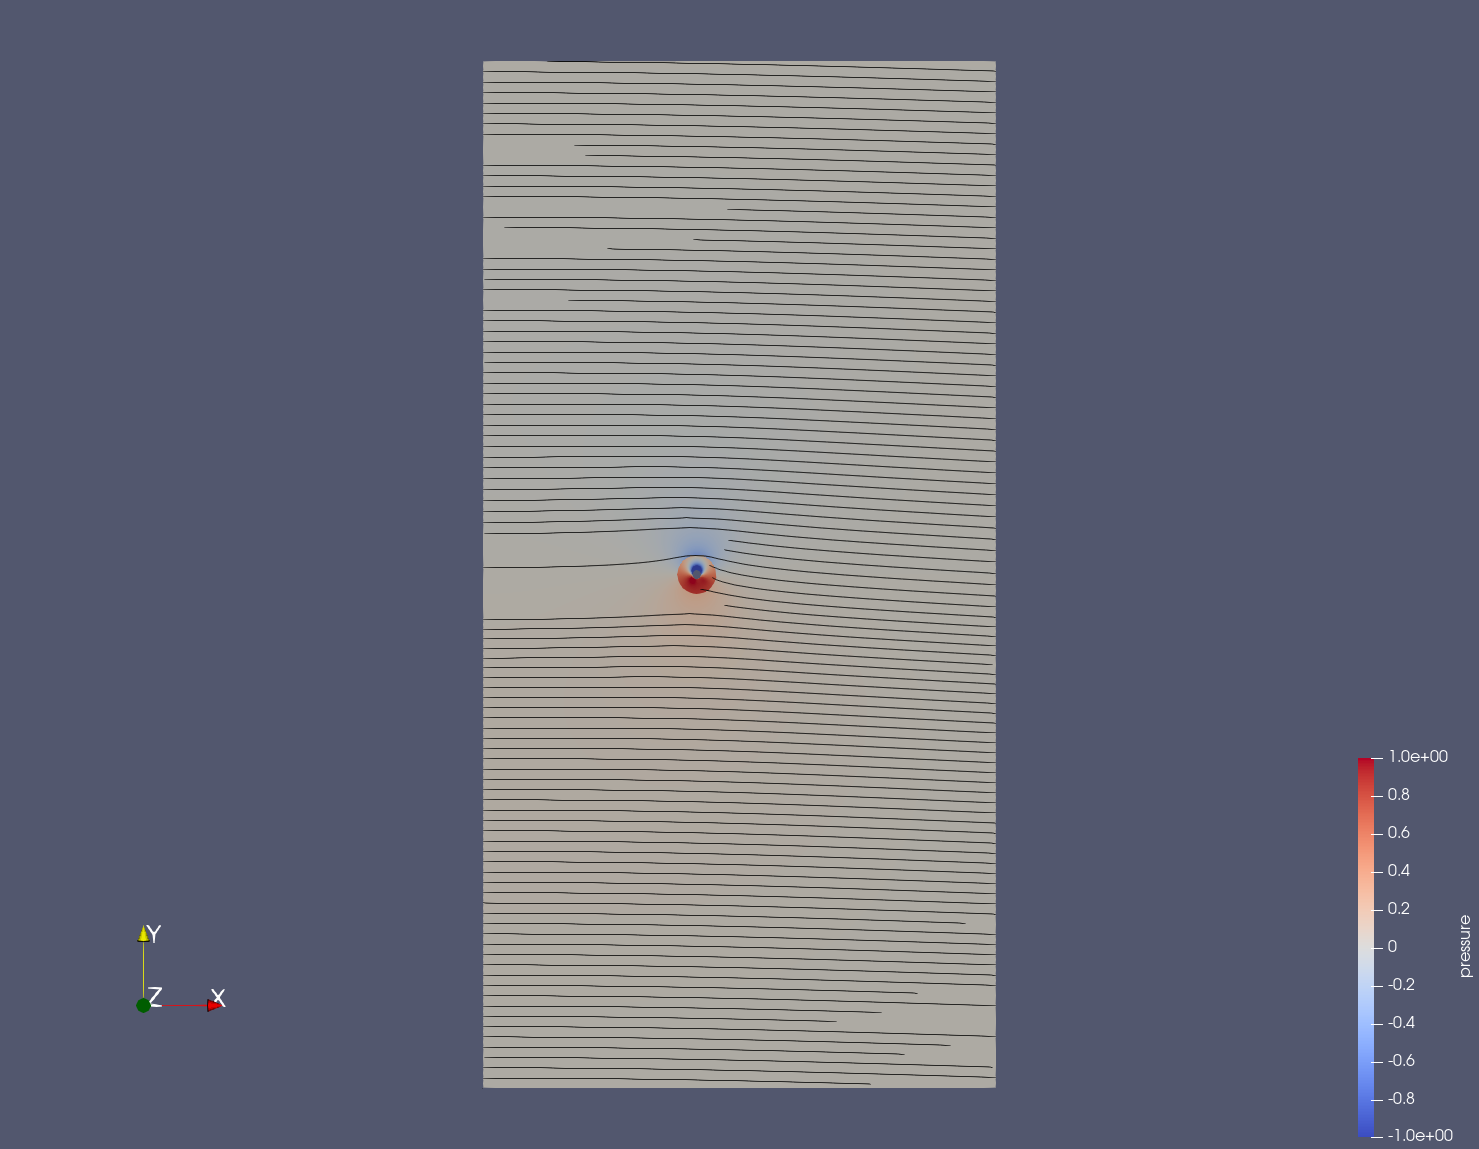
\includegraphics[width=\textwidth]{per12.png}
    \caption{Periodic boundary conditions}
    \label{fig:per12}
    \end{subfigure}
    \begin{subfigure}{0.49\textwidth}
    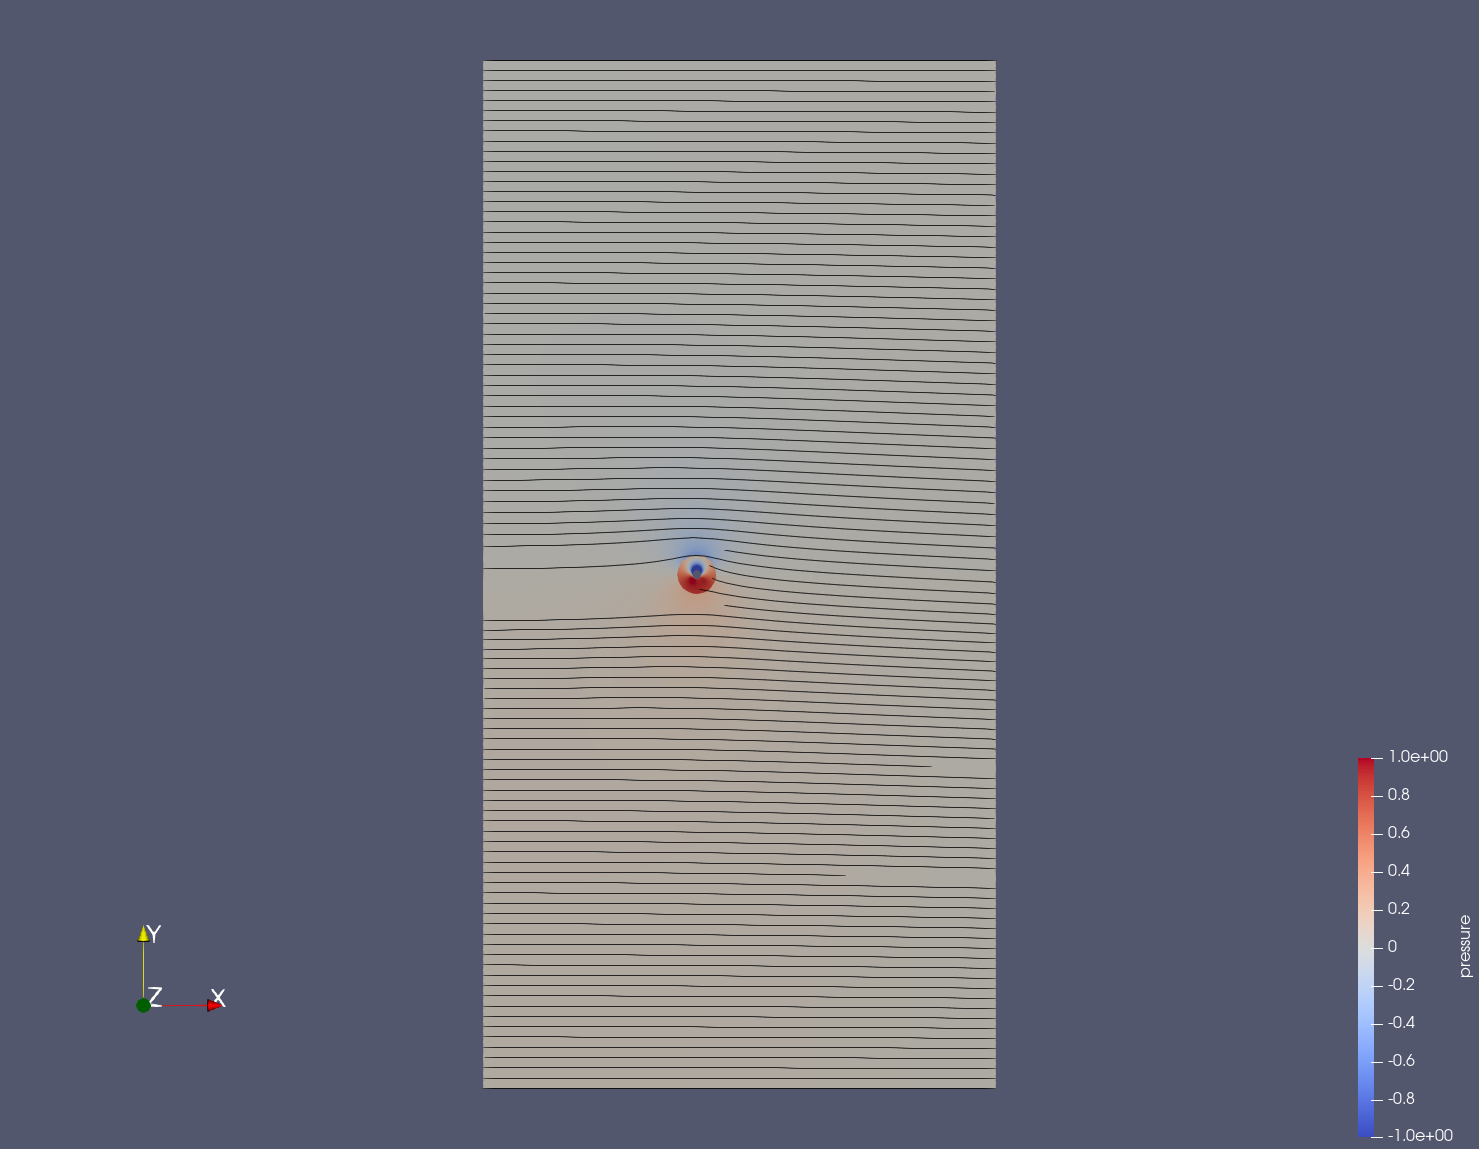
\includegraphics[width=\textwidth]{sym12.png}
    \caption{Symmetric boundary conditions}
    \label{fig:sym12}
    \end{subfigure}
    \caption{Pressure and streamline plots at $H=120D$, $\Omega^{\ast} = 3$, $\Rey = 200$, aspect ratio = 1}
    \label{fig:per sym12}
\end{figure}

Mittal and Kumar \cite{mittal_flow_2003} conducted a similar test looking only at symmetric boundary conditions. They conducted a study by varying the side length of a square mesh with a cylinder in the middle. They found that the drag values converge when the size of the domain is increased, which is consistent with our findings. However, their study changed both dimensions of the domain at the same time. Our study isolates the effect of the height of the domain. They did also find that lift is unaffected by domain size, which is consistent with our results. 

We ran our simulations with polynomial order $N = 11$. We ran a case with $N = 9, 11, 13$ which, on a grid of $E = 3712$ elements, correspond to gridpoint counts between $n = E \cdot 9^2 = 300,672$ and $n = E \cdot 13^2 = 627,328$. The change in drag is less than $1\%$ and the change in lift is less than $2\%$. The mesh independence cases were conducted on the $Fr^2 = 0.01$, $AR = 1.5$ case.


\section{Gravity wave analysis}
\label{section:IGW_analysis}
We intend to conduct an analyisis of the IGW that goes deeper than making qualitative observations based on timeseries and field plots. We intend to apply a Hilbert transform on the field plots in the same fashion that Mercier et al. \cite{mercier_reflection_2008} does. We do this to isolate the different waves using their respective wave numbers. We will first obtain data from the simulation fields by means of a structured gird, since our mesh is not a structured grid. We demodulate the field by applying a Fourier tranform, apply a filter, and then apply an inverse tranfrom. We are interested in the effects spin, aspect ratio, and stratification have on the IGW along the two directions. 